\documentclass[10pt,a4paper]{article}
\usepackage[margin=1.8cm]{geometry}
\usepackage{amsmath,amssymb}
\usepackage{booktabs}
\usepackage{graphicx}
\usepackage[T1]{fontenc}
\usepackage{microtype}
\usepackage[colorlinks,linkcolor=black,citecolor=black,urlcolor=blue]{hyperref}
\usepackage{xcolor}
\usepackage{tabularx}
% A GATE THAT PASSED IS GREEN AND A GATE THAT FAILED IS RED, in the table and nowhere else -- the
% colour is the verdict, so it is never spent on decoration.
\definecolor{gpass}{HTML}{1B7F4B}
\definecolor{gfail}{HTML}{B03A2E}
\newcommand{\pass}[1]{\textcolor{gpass}{\textbf{#1}}}
\newcommand{\fail}[1]{\textcolor{gfail}{\textbf{#1}}}
\newcolumntype{L}{>{\raggedright\arraybackslash}X}
\usepackage{titlesec}
\titlespacing*{\section}{0pt}{6pt}{2pt}
\newcommand{\code}[1]{\texttt{#1}}
\newcommand{\op}[1]{\texttt{#1}}
\title{\vspace{-1.4cm}\textbf{The vertex\,/\,MPM interface:\\
\normalsize a surface and a continuum exchanging force, and the spheroid it was built for}}
\author{}
\date{\vspace{-0.9cm}\small \texttt{prototype/ecm/mesh\_contact\_ops.py} $\cdot$
\texttt{test\_03\_mesh\_contact.py} $\cdot$ \texttt{test\_04\_spheroid\_ecm.py} $\cdot$
\texttt{gates\_03.py} $\cdot$
\texttt{log/okuda\_ECM/03*, 03d\_gates, 04*} $\cdot$ 10 August 2026}
\setlength{\parindent}{0pt}\setlength{\parskip}{0.55em}
\begin{document}\maketitle\vspace{-1.0cm}

\section*{1.\; Mechanism}

An epithelium pressing into a matrix is two materials touching: a sheet of cells that is a
\emph{surface} with no thickness worth resolving, and a stroma that is a \emph{continuum}. Everything
biological that happens between them --- adhesion, contact, load transmission, the slip that lets a
tissue slide over a gel instead of welding to it --- crosses that boundary, and it is a boundary
between two different kinds of object rather than between two materials.

\textbf{The obvious numerical scheme does not fit, and the reason is a ratio.} Outside biology this is
FEM--MPM coupling, and its natural form is \emph{grid-node} coupling (CFEMP \cite{lian2011}): resolve
contact by comparing the two bodies' velocities at grid nodes they share. It requires the mesh and the
grid to be comparable in size. Ours are not. A cell of this epithelium is $0.27$ to $0.42$ grid cells
across and a basement membrane is $0.1$, so both bodies fall inside one cell, the grid hands them a
single mass-weighted velocity, and they are \emph{welded} --- which is what runs 142--151 measured ten
times over. \emph{Particle-to-surface} coupling (ICFEMP \cite{chen2015}) removes the restriction by
testing a particle against a mesh \emph{face} rather than against a node, and that is the mechanism
here.

\textbf{What the mechanism has to carry, biologically.} Three things, and each is a term in \S2. A
\emph{normal} force, so the matrix is displaced rather than passed through. Its \emph{reaction}, so the
tissue feels what it pushes --- a one-way push is a decorative deformation, and the whole point of a
matrix that pushes back is that confinement becomes an outcome instead of a boundary condition.
And \emph{friction}, because a real epithelium slides against a gel: with no tangential law the shared
grid gives no-slip for free, and a "contact" that is MPM's automatic weld wearing a coefficient is not
a contact.

\section*{2.\; Equations and symbols}

For particle $p$ under face $f$, let $\hat{\mathbf n}$ be the face's outward normal and $\mathbf w$ the
barycentric weights of $p$'s contact point on it. The penetration, the normal penalty and the
regularised Coulomb friction are
%
\begin{align}
d_p &= \bigl[(\mathbf x_f-\mathbf x_p)\cdot\hat{\mathbf n}\bigr]_+,
&\mathbf f^{\,n}_p &= k\,d_p\,\hat{\mathbf n},
\label{eq:pen}\\[2pt]
\Delta\mathbf v_t &= \bigl(\mathbf v_p-\textstyle\sum_i w_i\mathbf v_i\bigr)_{\!\perp\hat{\mathbf n}},
&\mathbf f^{\,t}_p &= -\min\!\Bigl(\mu k d_p,\;\mu k d_p\tfrac{|\Delta\mathbf v_t|}{\varepsilon}\Bigr)
\frac{\Delta\mathbf v_t}{|\Delta\mathbf v_t|},
\label{eq:fric}
\end{align}
%
and the reaction is distributed to the face's vertices by the same weights, which is what makes the
exchange conservative by construction:
%
\begin{equation}
\mathbf f_i \;=\; -\,w_i\bigl(\mathbf f^{\,n}_p+\mathbf f^{\,t}_p\bigr),
\qquad\text{so}\qquad
\sum_p\mathbf f_p+\sum_i\mathbf f_i=\mathbf 0 .
\label{eq:reaction}
\end{equation}
%
$\varepsilon$ is a slip velocity and not a fudge: it is the speed below which a contact is treated as
stuck, so a resting contact does not chatter.

\textbf{Finding the face is a ray, and that is what makes it exact.} The tissue is star-shaped about
its own centroid, so the contact point is the intersection of the ray from the centroid through the
particle with the surface. M\"oller--Trumbore on triangle $(\mathbf A,\mathbf B,\mathbf C)$ gives the
weights and the surface radius $t$ in one solve:
%
\begin{equation}
t=\frac{\mathbf e_2\!\cdot\!\mathbf q}{\mathbf e_1\!\cdot\!\mathbf p},\quad
w_1=\frac{\mathbf s\!\cdot\!\mathbf p}{\mathbf e_1\!\cdot\!\mathbf p},\quad
w_2=\frac{\hat{\mathbf u}\!\cdot\!\mathbf q}{\mathbf e_1\!\cdot\!\mathbf p},
\qquad
\mathbf x_f=\mathbf c+t\,\hat{\mathbf u}_p,
\label{eq:mt}
\end{equation}
%
with $\mathbf e_{1,2}$ the triangle's edges from $\mathbf A$, $\mathbf s=\mathbf c-\mathbf A$,
$\mathbf p=\hat{\mathbf u}\times\mathbf e_2$, $\mathbf q=\mathbf s\times\mathbf e_1$. $t$ is the
curved-surface form of a flat patch's interpolated height, and the weights fall out of the same solve
rather than being a second, separate projection.

\textbf{The one constraint that is not optional.} The contact reaches the particle as a body force
integrated at $\Delta t$, so it is stable only while $\Delta t\sqrt{k/m}<1$:
%
\begin{equation}
k<k_{\max}=\frac{m}{\Delta t^2},
\qquad\text{written as}\qquad
k=\bigl(\code{k\_frac}/\Delta t\bigr)^2\ \text{in acceleration units}.
\label{eq:cfl}
\end{equation}
%
The first version of the flat rig used $k=3\times10^4$ against a ceiling of $95$, three hundred times
past it, and the same mistake NaN'd the flat sheet at $k=6\times10^3$. Writing the stiffness as a
\emph{fraction} of its own ceiling is what stops it being made a third time.

\smallskip
{\small\begin{tabular}{@{}llp{8.6cm}@{}}\toprule
symbol & is & of what\\\midrule
$d_p$ & penetration & of particle $p$ behind the face, along the face NORMAL, not along the ray\\
$k$ & penalty stiffness & in acceleration units; $\code{k\_frac}^2/\Delta t_{\rm sub}^2$, and
  $\code{k\_frac}=0.15$ throughout\\
$\mu$ & friction coefficient & Coulomb, regularised below $\varepsilon$\\
$\varepsilon$ & slip velocity & the speed below which a contact is stuck; $10^{-3}$\\
$\mathbf w$ & barycentric weights & of the contact point; they build the force AND distribute its
  reaction --- one array, so the two cannot disagree\\
$t$ & surface radius along the ray & Eq.~\eqref{eq:mt}; the star-shape's stand-in for a height\\
$\hat{\mathbf u}_p$ & particle direction & from the tissue centroid, which is also the bin key\\
\code{a\_max} & the operator's own clamp & applied BEFORE the reaction is recorded, so the momentum
  gate cannot pass on a force the scatter later clipped\\
\bottomrule\end{tabular}}

\section*{3.\; The Plexus2 container}

\textbf{Contact is a relation, so it is an edge set and not a force field on a body.}

\begin{center}\small
\begin{tabular}{@{}lll@{}}\toprule
\textbf{set} & \textbf{kind} & \textbf{state it carries}\\\midrule
\code{contact} & \textbf{edge}, \code{pre: mpm\_particle}, \code{post: vertex} & $d_p$, $\mathbf w$,
  the face, bound flag\\
\code{surface} & node set, one per membrane node & direction and radius --- \emph{deleted by this
  operator}, see below\\
\bottomrule\end{tabular}
\end{center}

\begin{center}\footnotesize
\begin{tabular}{@{}lllp{4.4cm}p{3.1cm}@{}}\toprule
\textbf{operator} & \textbf{kind} & \textbf{acts on} & \textbf{mechanism} & \textbf{its gate}\\\midrule
\op{contact\_rebuild} & \textbf{Rewire} & \code{contact} & which particle is under which face; the
  $(\theta,\phi)$ bin lookup & S1--S3\\
\op{mesh\_contact}    & \textbf{Lateral} & \code{contact} & Eqs.~\eqref{eq:pen}--\eqref{eq:reaction};
  returns a delta to \emph{both} endpoints in one call & S4--S8\\
\op{mesh\_inside\_count} & Lateral (diagnostic) & \code{mpm\_particle} & counts what is behind the
  surface; does not move it & S7\\
\bottomrule\end{tabular}
\end{center}

\textbf{The lookup, which is the only thing a curved surface needs that a flat one does not.} A
direction names the face. The bin structure is the one \op{apical\_map} already uses for
$R(\theta,\phi)$, holding the \emph{triangles} instead of a radius --- and that difference is the
operator: a bin of the map is a NUMBER, so it can only push radially and can return its reaction to
nothing, while a bin here holds three real vertices. Two details are not free. \textbf{The grid is
re-sized every frame}, because the nine-bin query is exact only while a triangle fits inside a bin and
the faces shrink from $0.17$ to $0.028$ rad as the tissue divides: $82$ bins in $8$ rows at frame $0$,
$3576$ in $53$ rows at the last, at most $64$ triangles in a bucket. And \textbf{the rows are
reduced} --- each given as many $\phi$ bins as it can hold \emph{square} ones,
$n_\phi=2\pi\sin\theta/\mathrm d\theta$ --- because on a plain $(\theta,\phi)$ lattice a bin near the
pole is a sliver, a triangle spans ten of them, and the query misses the face the particle is standing
on: silently, only near the poles, with matrix inside the tissue as the symptom.

\textbf{Placement, and it is worth $64\times$.} \op{mesh\_contact} goes \emph{inside} the
\code{substep\_dt} block, recomputed at the substep's own positions; at frame level the ceiling in
Eq.~\eqref{eq:cfl} falls by $(\Delta t_{\rm frame}/\Delta t_{\rm sub})^2$. The diagnostics go after it,
at frame level, because a non-penetration count must test this frame's positions against \emph{this}
frame's mesh.

\smallskip
{\footnotesize
\begin{verbatim}
  schedule:
    - aggregate -> seed_ecm
    - {substep_dt: 4.0e-4, steps: [mesh_contact, mpm_strain, mpm_scatter,
                                   mpm_grid_update, mpm_gather]}
    - ecm_stress -> mesh_inside_count
\end{verbatim}}
\smallskip

\textbf{What it deletes.} \op{cell\_to\_ecm[replay]}, a radial force read off a smoothed $32\times64$
radius map --- it cannot return a reaction (a bin has no vertices) and cannot generate a shear (a
radial force has no tangential part). And \op{cell\_exclude\_3d}, the projection backstop, because it
makes non-penetration \emph{unmeasurable}: with it on, the answer is zero by construction.

\section*{4.\; Gates}

A gate is a number with a threshold decided \emph{before} the run and a stated consequence if it
fails. S1--S3 run before any physics, as \code{mesh\_contact\_ops.selftest()}; a run refuses to start
if they fail. S12--S16 are the sweep no penalty method may skip: the stiffness, the time step and the
grid spacing are not physics, and a result that moves when they move is a result about the
discretisation.

\smallskip
{\scriptsize\setlength{\tabcolsep}{4pt}
\begin{tabularx}{\textwidth}{@{}llLl@{}}\toprule
& \textbf{gate} & \textbf{threshold} & \textbf{measured}\\\midrule
\multicolumn{4}{@{}l}{\textit{the lookup, before any physics} (meshes $0$, $100$, $199$)}\\
S1 & a ray from the centroid hits a closed star-shaped surface & coverage $>0.9999$ &
     \pass{1.00000} on all three\\
S2 & the binned face is the one a test against EVERY triangle finds & $0$ of $400$ rays &
     \pass{0}, max relative $0.0$\\
S3 & bucket occupancy stays bounded as the mesh refines & $<128$ per bucket &
     \pass{64} at $38{,}268$ triangles\\
\multicolumn{4}{@{}l}{\textit{the interface} (\op{03}, \op{03b}, \op{03c}; \op{04}, \op{04c/d})}\\
S4 & momentum: $|\sum\mathbf f_{\rm part}+\sum\mathbf f_{\rm vert}|/\sum|\mathbf f|$, flat patch &
     $<10^{-6}$ & \pass{1.5e-7} (float32 precision)\\
S5 & the same on a curved, dividing, re-meshed surface & $<10^{-6}$ & \pass{1.2e-7} max,
     \pass{1.5e-8} median\\
S6 & penetration stays bounded & $<2$ cells & \pass{1.47} (03b), \pass{0.82} (04), \pass{0.73} (04d)\\
S7 & particles behind the surface are the CONTACT, not a leak & ratio to particles in contact
     $<1.5$; none below $0.7R$ & \pass{0.90--0.96}; deepest \pass{0.90R}, \pass{0} below $0.7R$\\
S8 & friction changes the slip: $\mu=0.4$ against $\mu=0$ & $>2\times$ &
     \pass{5.3$\times$} (03b), \pass{3.9$\times$} (03c)\\
S9 & the operator's own clamp never binds & $\max a<\code{a\_max}$ & \pass{1.8e3} against $3\times10^4$\\
\multicolumn{4}{@{}l}{\textit{what the spheroid does to the matrix} (\op{04}, \op{04c}, \op{04d})}\\
S10& the far field is the bounded shell's own $C_1r+C_2/r^2$ & $R^2>0.90$ &
     \pass{0.94--0.999} (04, S/N $3.9$--$5.5$); \pass{0.88--0.998} (04c/d, S/N $1.9$--$2.9$)\\
S11& strand reorientation is its own affine control & within $5\%$ & $0.2725$ vs \pass{0.2714}\\
\multicolumn{4}{@{}l}{\textit{the discretisation} (\op{03d\_gates}, $1600$ frames, $k$ over $16\times$)}\\
S12& momentum residual in EVERY variant & $<10^{-6}$ & \pass{1.47--1.57e-7}\\
S13& penetration scales as $1/k$ & log-log slope in $[-1.4,-0.6]$ & \fail{-0.15}
     ($1.92\to1.27$ cells)\\
S14& the block's compression does not move with $k$ & spread $<0.10$ of nominal &
     \fail{0.119} ($13.88\to14.95\to15.66\%$)\\
S14b& the transmitted impulse does not move with $k$ & spread $<0.15$ of nominal & \fail{0.181}\\
S15& the answer is converged in the time step & compression within $0.05$ & \fail{0.237}
     ($14.95\to18.50\%$ at half the step)\\
S16& the interface does not consult the grid: $n_{\rm grid}$ $64\to96$ & compression within $0.15$,
     depth (box) within $0.5$ & \pass{0.123}; depth \pass{0.067}\\
\bottomrule\end{tabularx}}
\smallskip

\textbf{Two conventions make these mean what they say.} \textbf{The momentum residual is taken on the
contact's own force pair}, inside the substep and before anything else is added --- with a drive in the
sum it stops being a statement about the reaction. And \textbf{penetration is reported in box units as
well as in cells} across the grid sweep, because $\mathrm dx$ is exactly what changes there and cells
alone would report a grid dependence that is the unit.

\textbf{S13--S15 are the finding of this note, and they are a failure.} A penalty permits a depth
$d=f/k$, so a sixteenfold stiffening should divide the penetration by sixteen and leave the material's
compression alone. Measured, the penetration falls by $1.5\times$ and the compression \emph{rises} by
$13\%$. Both say the same thing: the depth is not set by a force balance but by how far the prescribed
surface advances before the penalty can accelerate a particle out of its way --- a rate-limited regime,
in which $k$ is not a numerical detail but part of the answer. S15 says the same thing from the time axis: halving the step
moves the compression from $14.95\%$ to $18.50\%$, so the run is not converged in $\Delta t$ either,
and for the same reason --- a rate-limited contact resolves more of the surface's advance when the
step is smaller. What survives untouched is S12, and S16 with it: the reaction is exact in every
variant, and refining the grid at fixed particle count moves the compression by $12\%$ and the
penetration in box units by $7\%$, which is the material's response and not the interface's --- the
one place the scheme's own claim, that particle-to-surface contact never consults the grid, is
tested and holds.

\textbf{What the gates license.} A surface and a continuum exchange force conservatively at a
resolution where grid-node coupling welds them (S4, S5); the slip is a material property rather than a
numerical accident (S8); the non-penetration the method fails to achieve is \emph{measured} rather
than projected away (S6, S7); and the matrix responds as the isotropic elastic shell it was given
(S10, S11). \textbf{What they do not license}: the quantitative contact --- S13 and S14 fail, so any
number that depends on how hard the surface pressed is provisional until the penalty is replaced by a
barrier formulation (BFEMP \cite{li2022}, which forbids penetration outright at the cost of an implicit
solve) or the press is made force-driven rather than displacement-driven. Nor two-way mechanics: the
tissue is still a replay, so the reaction it computes is recorded and dropped. Handing
\code{vertex\_force} to a live epithelium is a schedule change rather than an architecture change, and
it is the next run.

\begin{figure}[t]\centering
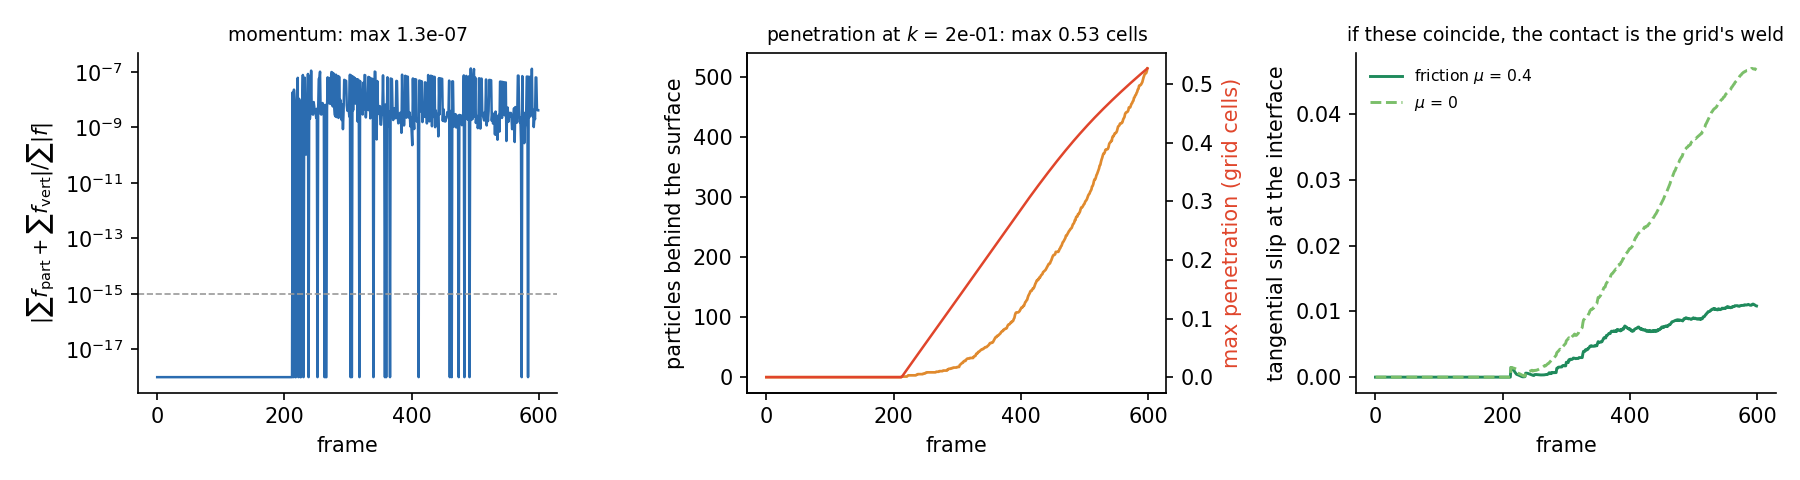
\includegraphics[width=\textwidth]{fig_mesh_contact_metrics.png}
\caption{\op{03}, the flat rig. \textbf{a} the momentum residual (S4), which a one-way coupling fails
by construction. \textbf{b} how many particles are behind the surface and how deep, in grid cells
(S6). \textbf{c} tangential slip with friction and without (S8) --- if these coincided, the contact
would be MPM's automatic weld wearing a friction coefficient.}
\end{figure}

\begin{figure}[t]\centering

\includegraphics[width=\textwidth]{../log/okuda_ECM/04d_spheroid_fibres/strip.png}
\caption{\op{04d}, the section, coloured by von Mises stress on one scale over the whole run. The
spheroid clears a hole in the matrix and a shell of compacted, stressed strands travels outward ahead
of it while the far field stays unloaded; the matrix nearest the tissue reaches $1.25$ times its own
seeded density at $r=0.158$, just outside the surface. First contact is frame $32$ of $400$, where the
cavity radius and the tissue radius cross.}
\end{figure}

\section*{5.\; References}

{\small
\begin{thebibliography}{99}\setlength{\itemsep}{0pt}
\bibitem{lian2011} Lian, Y.P., Zhang, X., Liu, Y. (2011) Coupling of finite element method with
material point method by local multi-mesh contact method. \emph{Comput. Methods Appl. Mech. Eng.}
\textbf{200}:3482--3494.
\bibitem{chen2015} Chen, Z.-P., Qiu, X.-M., Zhang, X., Lian, Y.-P. (2015) Improved coupling of finite
element method with material point method based on a particle-to-surface contact algorithm.
\emph{Comput. Methods Appl. Mech. Eng.} \textbf{293}:1--19.
\bibitem{li2022} Li, X., Fang, Y., Li, M., Jiang, C. (2022) BFEMP: Interpenetration-free MPM--FEM
coupling with barrier contact. \emph{Comput. Methods Appl. Mech. Eng.} \textbf{390}:114350.
\bibitem{moller1997} M\"oller, T., Trumbore, B. (1997) Fast, minimum storage ray/triangle
intersection. \emph{J. Graphics Tools} \textbf{2}(1):21--28.
\bibitem{okuda2018} Okuda, S., Miura, T., Inoue, Y., Adachi, T., Eiraku, M. (2018) Combining Turing
and 3D vertex models reproduces autonomous multicellular morphogenesis. \emph{Sci. Rep.} \textbf{8}:2386.
\bibitem{hu2018} Hu, Y. \emph{et al.} (2018) A moving least squares material point method with
displacement discontinuity and two-way rigid body coupling. \emph{ACM Trans. Graph.} \textbf{37}(4):150.
\bibitem{wang2014} Wang, H., Abhilash, A.S., Chen, C.S., Wells, R.G., Shenoy, V.B. (2014) Long-range
force transmission in fibrous matrices enabled by tension-driven alignment of fibers.
\emph{Biophys. J.} \textbf{107}(11):2592--2603.
\end{thebibliography}}

\end{document}
